\documentclass[a4paper, 12pt,oneside]{article} 
%\documentclass[a4paper, 12pt,oneside,draft]{article} 

\usepackage{preamble}
\usepackage{bm}
%--------------------- ACTUAL FILE ---------------------- %
\begin{document} 
	\begin{center}
	    \Large
	    \textbf{Project 5 : Causal discovery}
	        
	    \vspace{0.4cm}
	    \large
	    Author : Tara Fjellman \\
	    \small{Spring 2024}
	\end{center}

    \section{Introduction}
    In this report we compare different methods to do causal discovery on the LUCAS0 artificially generated lung cancer data set. We do so in the context of then running a logistic regression for the lung cancer target variable $T$, in terms of other variables given for each data entry. 
    We aim to investigate whether the Incremental Association Markov Blanket (IAMB) performs better than a simpler PC algorithm at recovering $T$'s Markov blanket. As baselines, we also include ground truth and LASSO\footnote[1]{When we refer to LASSO in this report, we actually mean L1 norm penalised logistic regression that uses likelihood maximisation as a cross validation metric.} variable selections. 

    To study the stability of the methods we also vary the size of the training set.  
    \section{Data exploration}
    The 11 covariates considered are binary ones. They respectively refer to : weather the person smokes, has yellow fingers, has anxiety, feels peer pressure, is genetically predisposed to develop cancer, has an attention disorder, is born on an even day, has had a car accident, experiences fatigue, has allergies, coughs.  
    
    The most unbalanced variables are the ones related to genetic predisposition and yellow fingers, where one of the classes have respective frequencies of 0.147 and 0.226. 

    We expect the unbalanced data to have a greater impact on the performance for smaller training set sizes.
    \section{Methods}
        \subsection{IAMB explanation}
        The algorithm  consists of two phases, a forward and a backward one. 
        In the forward phase all variables that have some degree of association with T are added to an initial guess $G$ for the Markov blanket. This is done sequentially, considering the mutual information conditioned on the current state of $G$. In the backward phase, the features are one-by-one tested for independence of T given the others. They are removed if they are found to be independent at significance level $\alpha$.
        This procedure is expected to recover T's Markov blanket as : (a) by definition it is the minimal set such that every variable in it is dependent on T given any of its subsets; (b) we make the faithfulness assumption (the underlying conditional independencies in the data imply conditional independencies in the DAG).
        \subsection{Dealing with stochastic outputs}
        During the experimentation we noticed that the results for all the tested algorithms depended strongly on the random seed used during sampling. To account for this, we decided to report the results under distributional form, by running the experiments $n_{\text{rep}}$ times and reporting the proportion of times in which the covariates were included in the Markov blanket. 
        \subsection{Regression evaluation}
        Once the Markov blanket is found, we run a logistic regression on the training set with the selected features. We then evaluate the performance of the models on the test set using the BIC and AUC score. The tested models are selected by looking at the distribution of the Markov blanket over the $n_{\text{rep}}$ repetitions. They are then further compared to the ground truth through likelihood ratio tests.
    \section{Training size sensitivity}
    In this section we study the sensitivity of the algorithms to the size of the training set. We vary the training set size from 100 to 1000, and observe the associated distributional shifts.
    The results for the IAMB and PC algorithms are shown in \ref{fig:mb-trainsize-sensitivity} while those associated to LASSO are in \ref{fig:lasso-trainsize-sensitivity}.
    \begin{figure}[h!]
        \centering
        \vspace{0em}
        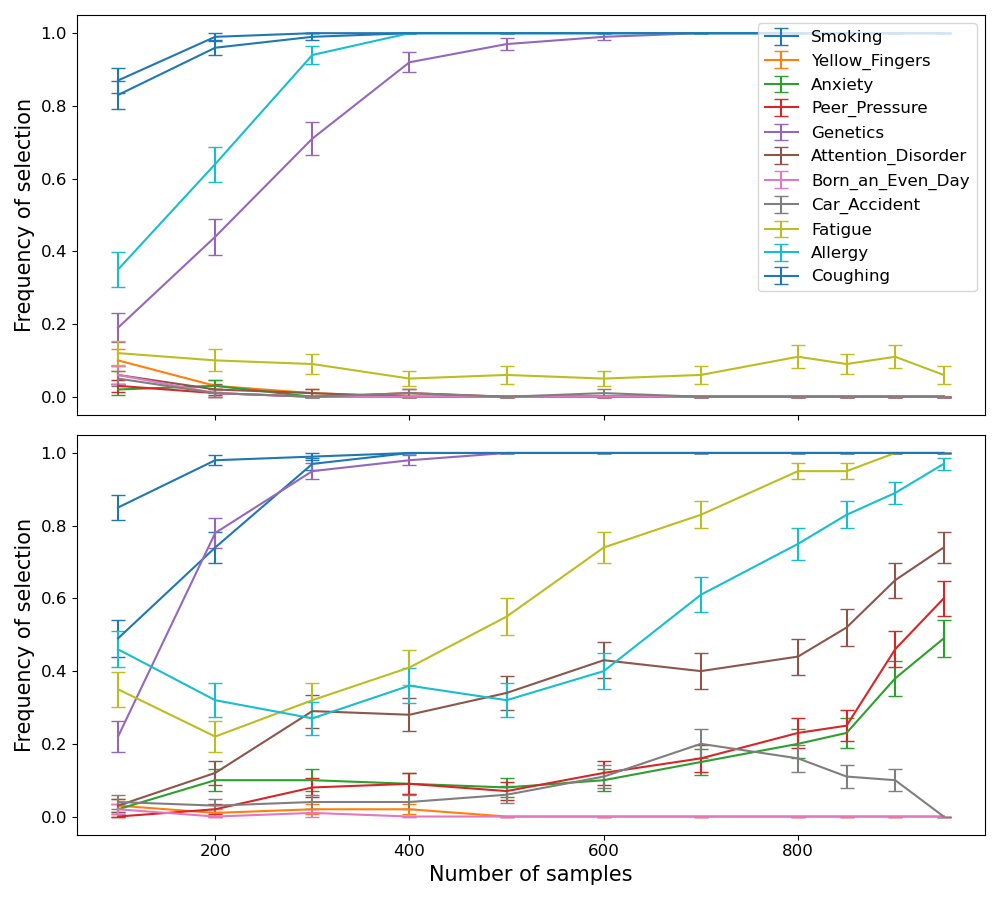
\includegraphics[width=.85\textwidth]{mb-trainsize-sensitivity}
        \caption{Evolution of the frequencies of selection for all the covariates as a function of training set size. The top figure is associated to the IAMB method while the bottom one is associated to PC method.}
        \label{fig:mb-trainsize-sensitivity}
    \end{figure}
    Looking at the first figure, it is apparent that IAMB and PC have vastly different behaviours. 
    
    IAMB excludes the variables that are outside the Markov blanket with high probability (for all training set sizes) and includes 4 of the 5 true variables with increasing probability. We can therefore say it performs better with higher training set sizes, as one would expect. It however includes the remaining true covariate, fatigue, only about 10\% of the time.
    
    On the other hand, PC includes most variables with increasing probability. This is beneficial for the inclusion of the fatigue covariate for example but problematic for the variables which are not not in the true Markov blanket such as peer pressure. This tendency leads to a decrease in performance with increasing training set size, which is unexpected. When compared to the LASSO results it should however still be preferred. Indeed, though the variables from the true Markov blanket are included with high (and highest) probability, all the other variables are also included with large probabilities. Its performance also does not clearly improve with data size.
    \begin{figure}[h!]
        \centering
        \vspace{0em}
        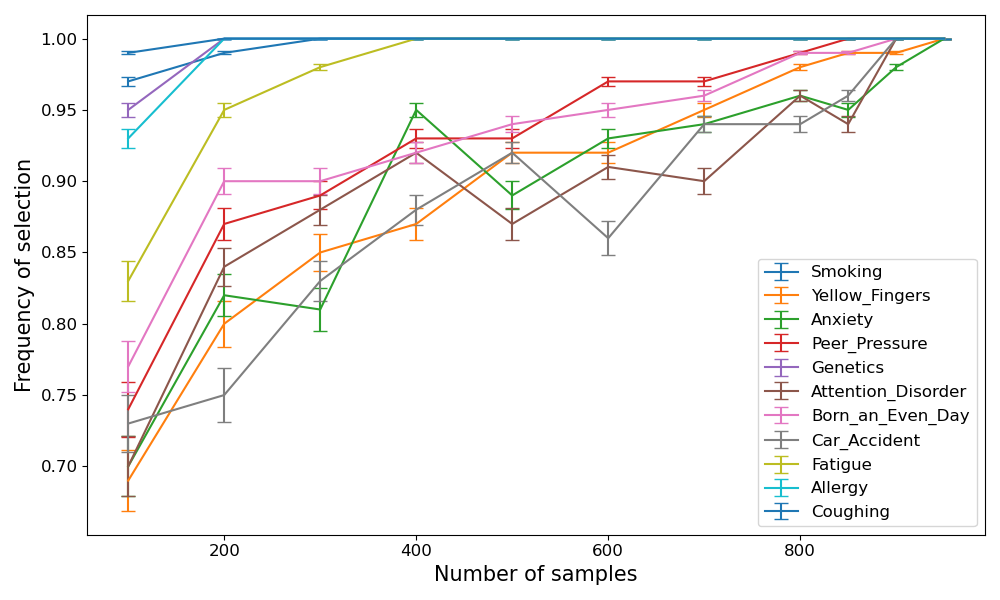
\includegraphics[width=.85\textwidth]{lasso-trainsize-sensitivity}
        \caption{Evolution of the frequencies of selection for all the covariates as a function of training set size. These results are associated to the LASSO selection.}
        \label{fig:lasso-trainsize-sensitivity}
    \end{figure}
    \section{Regression results}
    The goal of this section is to explore the impact of mis-estimating the Markov blanket in the context of logistic regression. To make the analysis concise, we only consider a few models that are representative of the different behaviours observed in the previous section. We consider the following models:
    \begin{itemize}
        \item The ground truth model, which includes the true Markov blanket.
        \item The no-fatigue model, which includes the true Markov blanket except for the fatigue.
        \item The no-allergy model, which includes the true Markov blanket except for the allergy.
        \item The full model, which includes all the covariates. 
    \end{itemize}
    For each of these models, we run a logistic regression on the training set, while BIC and AUC score are computed on the test set. The results are shown in \ref{tab:regression-results}.
        \begin{figure}[h!]
        \centering
        \vspace{0em}
        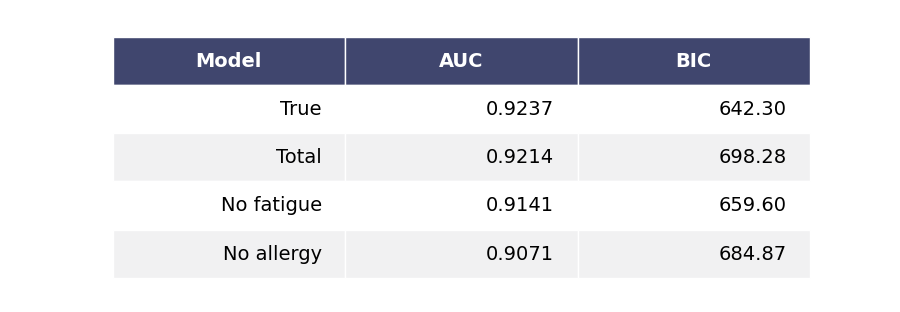
\includegraphics[width=.6\textwidth]{regression-results}
        \caption{Regression metrics for different models. These are obtained by training the logistic regression on the full training set and evaluating the metrics on the test set.}
        \label{tab:regression-results}
    \end{figure}
    The table suggests that the full model over-fits the data, as it has by far the highest BIC. This is also confirmed by the AUC score which is not larger than for the true model and the 0.273 p-value associated to the full vs true likelihood ratio test. 
    On the other side, the models where one of the true covariates is excluded under-fit the data. This can be seen by the lower AUC score,the higher BIC and the fact that the p-values for the true vs nested likelihood ratio tests are significant at 3.45e-4 and 5.17e-14 respectively. Notice that these results also suggest that the fatigue variable is less important than the allergy one, which might explain partly why the IAMB algorithm had a hard time including it in the Markov blanket.
    \section{Conclusion}
    In this report we have compared the IAMB and PC algorithms for causal discovery on the LUCAS0 data set. We have found that the IAMB algorithm is more stable and performs better than the PC algorithm, but however did not include one of the variables of the Markov blanket with high probability. When compared to the use of LASSO, PC was still found to be preferable. Except for the IAMB algorithm, the performance was surprisingly not found to improve increasing size of the training set. Based on this report, the use of the IAMB algorithm seems to be a good option for doing causal discovery. A deeper study to explore the reasons for which the fatigue variable was not included in the Markov blanket is however needed. When it comes to the regression, the results suggest that using the Markov blanket avoided over and under fitting. % could add remark about computational cost
    \section*{Appendix}
    This appendix contains the plots associated to the variable selection that was made using LASSO. The goal is to show that LASSO shrinks the the coefficients of the variables that are not in the Markov blanket to zero before the ones that are within it (see \ref{fig:lasso-coef-path}). The problem with the method therefore lies in the fact that the regularisations associated to this behaviour is not preferred over the one that includes all the variables (see \ref{fig:lasso-likelihood-path}).
    \begin{figure}[h!]
        \centering
        \vspace{0em}
        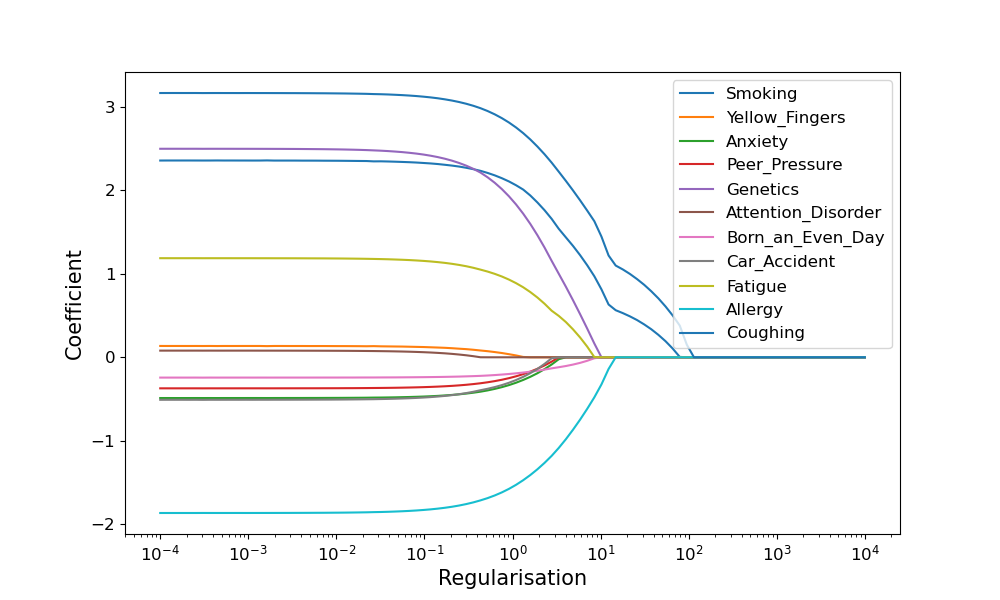
\includegraphics[width=.95\textwidth]{lasso_coef_path}
        \caption{Coefficient paths of associated to the LASSO variable selection. Here the training size is taken as $n=500$.}
        \label{fig:lasso-coef-path}
    \end{figure}
    \begin{figure}[h!]
        \centering
        \vspace{0em}
        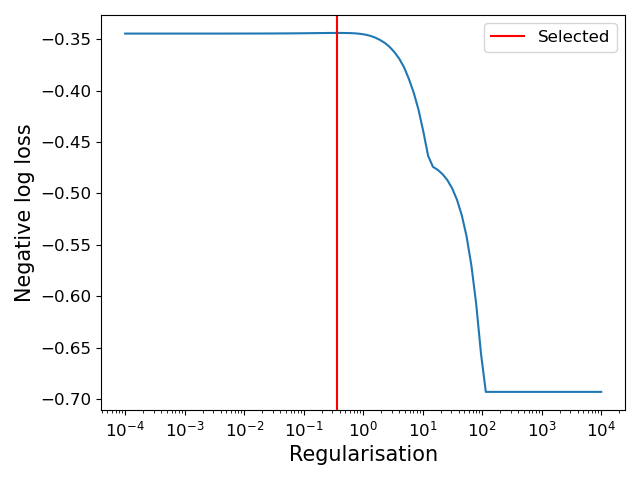
\includegraphics[width=.65\textwidth]{lasso_likelihood_path}
        \caption{Validation curve (average over the folds). The red line corresponds to the regularisation maximising the likelihood. Here the training size is taken as $n=500$.}
        \label{fig:lasso-likelihood-path}
    \end{figure}
    \section*{Acknowledgements}
    I thank Rayan Harfouche for discussions during and outside the exercise sessions.
    \section*{References}
    [1] I. Tsamardinos, C. F. Aliferis, and A. Statnikov, ‘Algorithms for Large Scale Markov Blanket Discovery’.

    [2] ‘LUCAS’. Accessed: May 05, 2024. [Online]. \newline Available: https://www.causality.inf.ethz.ch/Fdata/LUCAS.html
\end{document}